% Supplementary material for the ToG double-anonymous submission.
% Every float below is relocated VERBATIM from the main manuscript
% (see PORT_TRIM_REPORT.md); only the S-prefix numbering and the two
% box-title labels are changed, each logged. Not counted toward the
% 10-page limit per ToG policy.

\documentclass[journal,onecolumn]{IEEEtran}

\usepackage[utf8]{inputenc}
\usepackage{microtype}
\usepackage{amsmath}
\usepackage{amssymb}
\usepackage{xcolor}
\definecolor{scienceRed}{HTML}{C8102E}
\definecolor{scienceRule}{HTML}{BBBBBB}
\definecolor{darkGray}{HTML}{333333}
\newcommand{\arch}[1]{\textbf{#1}}
\usepackage{graphicx}
\graphicspath{{figures/}{./}}
\usepackage{float}
\usepackage{booktabs}
\usepackage{array}
\usepackage{tabularx}
\usepackage{multirow}
\usepackage[most]{tcolorbox}
\tcbset{
  storyhand/.style={
    enhanced, breakable=false, boxrule=0.4pt, arc=2pt,
    colback=gray!3, colframe=scienceRed!70,
    coltitle=white, colbacktitle=scienceRed,
    fonttitle=\sffamily\bfseries\fontsize{9}{11}\selectfont,
    title={#1},
    left=8pt, right=8pt, top=6pt, bottom=6pt,
    boxsep=3pt,
  }
}
\usepackage{xurl}
\usepackage[colorlinks=true,
            linkcolor=black,
            citecolor=scienceRed,
            urlcolor=scienceRed!80!black]{hyperref}

% Supplementary numbering
\renewcommand{\thetable}{S\arabic{table}}
\renewcommand{\thefigure}{S\arabic{figure}}

\title{Supplementary Material for ``Trust Dynamics in Multi-Agent
  Strategic Interaction: A Simulation Study of Bayesian Reputation
  Systems in 8-Player Limit Texas Hold'em''}
\author{Anonymous authors}

\begin{document}
\maketitle

\begin{table*}[t]
\centering
\caption{\textbf{A primer on fixed-limit Texas Hold'em.} The
minimum set of concepts needed to read the rest of the paper. The
betting bounds in the ``Bet sizing'' row are the specific values
we use throughout the simulation; everything else applies to
fixed-limit Hold'em in general.}
\label{tab:poker-primer}
\small
\begin{tabularx}{\textwidth}{@{}lX@{}}
\toprule
Concept & Description \\
\midrule
Hole cards & The two private cards each player is dealt at the start of every hand; only that player can see them. \\
Community cards & Up to five face-up cards shared by everyone at the table; players combine these with their hole cards to form a 5-card hand. \\
Betting rounds & Four sequential rounds per hand: preflop (no community cards yet), flop (three community cards revealed), turn (one more), and river (the fifth and final). \\
Actions & At each turn a player may fold (give up the hand), check (pass without betting, only if no one has bet), call (match the current bet), bet (open the wagering), or raise (increase an existing bet). \\
Bet sizing (this paper) & Small bet 2 chips on preflop and flop; big bet 4 chips on turn and river; no more than four raises per round (the ``four-bet cap''). \\
Blinds & Forced bets: small blind 1 chip and big blind 2 chips, posted by the two seats clockwise of the dealer and rotating each hand. \\
Pot & The accumulated chips at stake in a hand. The winner of the hand collects the pot. \\
Showdown & End-of-hand reveal: surviving players turn over their hole cards and the strongest 5-card combination wins. A hand that ends with everyone folding never reaches showdown. \\
Stack & The chips a player has in front of them; depleting to zero triggers a rebuy in our setup. \\
\bottomrule
\end{tabularx}
\end{table*}

\begin{figure}[!ht]
  \centering
  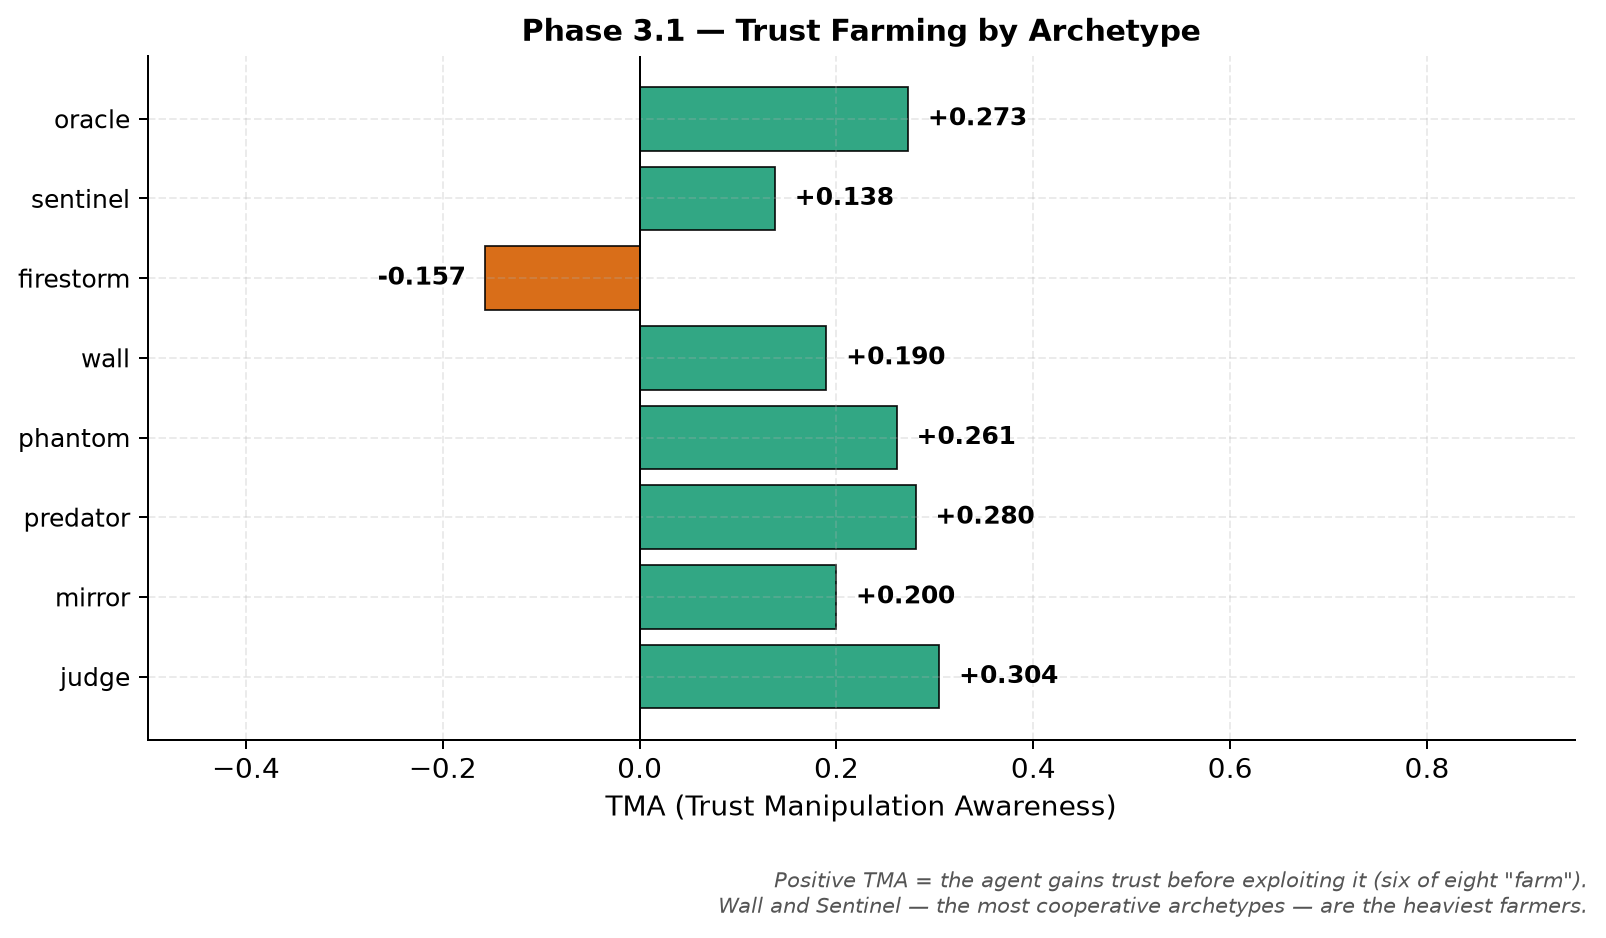
\includegraphics[width=\linewidth]{06_tma_by_archetype.png}
  \caption{\textbf{Trust Manipulation Awareness (TMA) per
  archetype in Phase 3.1.} Positive TMA indicates an agent's
  rolling trust delta correlates with its rolling aggression delta---building trust through cooperative early play, then leveraging it for higher-aggression later moves. Seven of eight archetypes show weakly positive TMA; \arch{Judge} ($+0.30$) and \arch{Predator} ($+0.28$) are the strongest.}
  \label{fig:tma}
\end{figure}

\begin{tcolorbox}[storyhand={Supplementary Box~S1.\quad An instance of the trap (Phase 3 hand \#67, 30 actions, 110-chip pot)}]
\scriptsize
\textbf{Setup.} Seed 42, hand 67. \arch{Wall} (seat 3) is dealt
$2\spadesuit\,5\clubsuit$ -- rank 6{,}749, the worst hand at the
table. Final pot 110 chips, showdown.

\smallskip
\noindent\textbf{Action sequence:}\par\nopagebreak
\begin{center}
\setlength{\tabcolsep}{3pt}\begin{tabularx}{\linewidth}{@{}rlllrr>{\raggedright\arraybackslash}X@{}}
\toprule
Seq & Seat & Round & Action & Amt & Pot & Notes \\
\midrule
 3 & \arch{Judge}     & preflop & raise & 4 & 7   &  \\
 6 & \arch{Firestorm} & preflop & raise & 6 & 13  & 3-bet \\
 7 & \arch{Wall}      & preflop & call  & 5 & 18  & \textit{calls 3-bet pot with 2-5 off} \\
 9 & \arch{Judge}     & preflop & call  & 2 & 20  &  \\
10--16 & \ldots & flop  & \ldots &   & 38  & \arch{Judge} bets, \arch{Firestorm} raises, \arch{Wall} calls each street \\
17--23 & \ldots & turn  & \ldots &   & 74  & Same pattern \\
24--30 & \ldots & river & \ldots &   & 110 & \arch{Wall} calls the final two raises \\
\bottomrule
\end{tabularx}
\end{center}

\smallskip
\noindent\textbf{Showdown.}
\arch{Firestorm} $J\heartsuit\,J\diamondsuit$ (rank 4042)
\textbf{wins} 110.
\arch{Judge} $8\heartsuit\,8\diamondsuit$ (rank 4703).
\arch{Wall} $2\spadesuit\,5\clubsuit$ (rank 6749).
\textit{Wall pays 35 chips into a hand it had no chance to win.
Every observer's posterior saturates near its ceiling---just short
of $1$, given the $\varepsilon$ noise floor---on \arch{Firestorm}
being a firestorm and on \arch{Wall} being a wall.}
\end{tcolorbox}

\begin{tcolorbox}[storyhand={Supplementary Box~S2.\quad The inversion in a single hand (original five-seed Phase 3.1 exploration, hand \#146, 17 actions, 32-chip pot)}]
\scriptsize
\textbf{Setup.} Seed 42, hand 146. \arch{Wall} (seat 3) is dealt
$K\heartsuit\,Q\heartsuit$ -- rank 872, a strong hand. Final pot
32 chips, showdown.

\smallskip
\noindent\textbf{Action sequence:}\par\nopagebreak
\begin{center}
\setlength{\tabcolsep}{3pt}\begin{tabularx}{\linewidth}{@{}rlllrr>{\raggedright\arraybackslash}X@{}}
\toprule
Seq & Seat & Round & Action & Amt & Pot & Notes \\
\midrule
 7 & \arch{Firestorm} & preflop & raise          & 3 & 10 &  \\
 8 & \arch{Wall}      & preflop & call           & 2 & 12 & calls 3-bet with K-Q suited \\
11 & \arch{Firestorm} & flop    & bet            & 2 & 14 & c-bet \\
12 & \arch{Wall}      & flop    & call           & 2 & 16 &  \\
13 & \arch{Firestorm} & turn    & bet            & 4 & 20 & second barrel \\
14 & \arch{Wall}      & turn    & call           & 4 & 24 &  \\
15 & \arch{Firestorm} & river   & \textbf{check} & 0 & 24 & \textit{tell --- bluff line abandoned} \\
16 & \arch{Wall}      & river   & \textbf{bet}   & 4 & 28 & \textit{value bet against checked range} \\
17 & \arch{Firestorm} & river   & call           & 4 & 32 &  \\
\bottomrule
\end{tabularx}
\end{center}

\smallskip
\noindent\textbf{Showdown.}
\arch{Wall} $K\heartsuit\,Q\heartsuit$ (rank 872) \textbf{wins} 32.
\arch{Firestorm} $8\clubsuit\,Q\clubsuit$ (rank 6075).
\textit{Canonical \arch{Wall} never bets the river in any Phase 1,
Phase 2, or Phase 3 dataset; Phase 3.1 \arch{Wall}, augmented with
chain-of-thought, per-opponent memory, and adaptive strategy
notes, does.}
\end{tcolorbox}

\section*{Broader Impact Statement}
This research examines ways in which an observation-based reputation system creates incentives for an agent to exploit its predictability with respect to cooperative behavior. Therefore, the mechanisms identified in this work can be used to develop a theoretical basis for discovering, modeling, or strategically leveraging trust in reputation systems. In particular, both the Trust Manipulation Awareness (TMA) metric and the concept of ``trust farming'' can be viewed as a conceptual approach for maximizing the use of trust instead of detecting it.

However, we believe that the practical risk of such misuse is limited by the scope of the findings presented here. All of our experiments were conducted in a synthetic, zero-sum game, and we continually argue throughout the paper that we should not infer direct application to real-world, positive-sum reputation systems. Instead, our results describe qualitatively, at a mechanism level, what appears to happen under the conditions studied rather than providing a specific deployable tactic against any existing marketplace, credit, or social reputation system. Each of those systems contains built-in institutional and enforcement mechanisms which were omitted from our testbed.

It is necessary to understand how an agent's ability to act cooperatively can be exploited in order to build systems that will resist such exploitation. Our results indicate that observation-based reputation systems have blind spots where agents possess overlapping behavioral profiles, and that defending cooperative agents may necessitate developing defense systems capable of reasoning beyond merely increasing the amount of observational information available. We thus consider this work as contributing toward understanding and mitigating mechanisms for exploiting trust as opposed to being an instrument for performing such exploitation. To facilitate greater scrutiny and replication, all experiments are fully specified and seeded, and the source code and raw data are available for public review.

\section*{Supplementary Materials}
The following supporting materials are available in the project
repository:
\footnotesize\raggedright
\begin{enumerate}\setlength{\itemsep}{2pt}\setlength{\parskip}{0pt}\setlength{\leftmargini}{1.5em}
  \item \textbf{Bayesian update worked example.} \path{docs/worked_examples.md}
  \item \textbf{Identifiability ceiling derivation.} \path{docs/stage5_identifiability.md}
  \item \textbf{Phase 2$^{*}$ unbounded-optimization methodology.} \path{paper_resources/notes/phase2_unbounded_writeup_aggressive.md}
  \item \textbf{Methods disclosures} (sampling temperature, side-pot construction, confidence intervals). \path{paper_resources/notes/methods_disclosures.md}
  \item \textbf{Bootstrap and Fisher-$z$ CI table.} \path{paper_resources/data/r_bootstrap_ci.csv}
\end{enumerate}

\end{document}
